\subsection{Web application}
	La componente \glock{web app} ha il compito di interfacciare gli utenti con i dispositivi censiti dal sistema e visibili al loro \glock{ente} di appartenenza.
	\newline
	Le principali funzionalità messe a disposizione riguardano la visualizzazione di grafici contenenti i dati di determinati sensori, la modifica delle configurazioni dei gateway e l'aggiunta o la rimozione di dispositivi e/o sensori.
	\newline 
	La componente è stata sviluppata utilizzando i \glock{framework Laravel} e \glock{Vue.js}.
	
	\subsubsection{Diagramma dei package}%%%%%%%%%OK
		\begin{figure}[H]
			\centering
			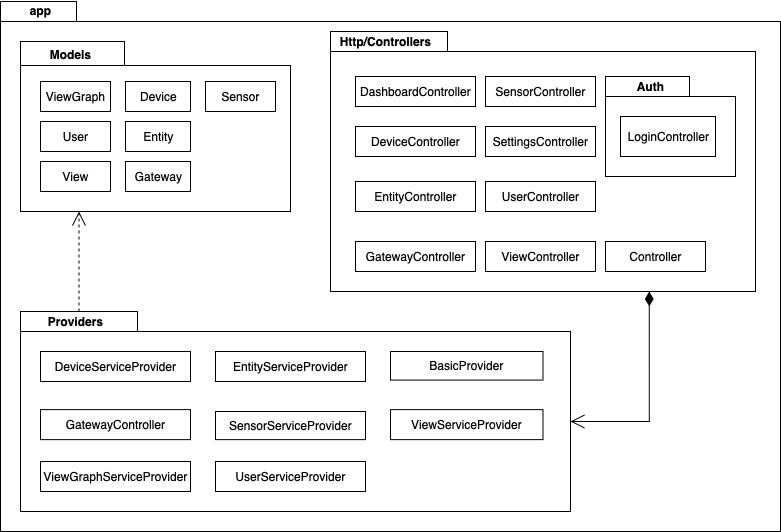
\includegraphics[scale=0.450]{res/images/WEBAPP/WebAppPackage.png}
			\caption{Diagramma dei package della componente web app}
			\label{Diagramma 21}
		\end{figure}
	
	\subsubsection{Dipendenze esterne}
		La componente ha le seguenti dipendenze esterne:
		\begin{itemize}
			\item \textbf{Laravel:} framework alla base della \glock{web app}, da cui vengono prese le basi dei controllers e dei models. Inoltre è il gestore delle view;
			\item \textbf{Laravel/UI:} viene utilizzata per l'autenticazione all'interno della web app;
			\item \textbf{guzzlehttp/guzzle:} viene utilizzata per effettuare richieste HTTP in linguaggio PHP;
			\item \textbf{Axios:} viene utilizzata per effettuare delle richieste HTTP in \glock{JavaScript};
			\item \textbf{Datatables.js:} viene utilizzata per la paginazione delle tabelle;
			\item \textbf{Apexcharts:} viene utilizzata per fare i grafici visibili all'interno dell'applicazione web;
			\item \textbf{davejamesmiller/laravel-breadcrumbs:} questa dipendenza viene utilizzata per generare i breadcrumb all'interno delle pagine visualizzate;
			\item \textbf{Vue.js:} framework che permette, tra le altre cose, di utilizzare array e variabili all'interno delle pagine per permetterne una visualizzazione dinamica dei contenuti;
			\item \textbf{Bootstrap:} framework utilizzato per la creazione dell'interfaccia grafica dell'applicazione web;
			\item \textbf{JQuery:} libreria utilizzata da \glock{Bootstrap} per molte delle sue componenti;
			\item \textbf{Popper.js:} altra libreria utilizzata da \glock{Bootstrap}.
		\end{itemize}



	\subsubsection{Diagrammi delle classi}%%%%%%%%%%OK
	Nel diagramma delle classi della componente \glock{web app}, rappresentato nel file \textit{Immagini/WebApp-Classi.png}, sono presenti principalmente i provider ed i controller: i provider sono le componenti che effettuano le richieste \glock{API} da parte della web app e lavorano quindi a basso livello.
	\newline
	I controller invece dialogano con i provider ad un livello di astrazione più alto. Le pagine view non sono presenti in quanto il framework \glock{Laravel} le gestisce tramite pagine HTML.
	Le classi presenti nel diagramma sono quindi:
	\begin{itemize}
		\item \textbf{Model}: tutte le classi che rappresentano un oggetto estendono la classe Model:
		\begin{itemize}
			\item \textbf{User}: questa classe rappresenta gli utenti del sistema;
			\item \textbf{Entity}: questa classe rappresenta gli enti presenti nel sistema;
			\item \textbf{Gateway}: questa classe rappresenta i gateway presenti nel sistema;
			\item \textbf{Device}: questa classe rappresenta i dispositivi presenti nel sistema;
			\item \textbf{Sensor}: questa classe rappresenta i sensori presenti nel sistema;
			\item \textbf{ViewGraph}: questa classe rappresenta i grafici presenti nel sistema;
			\item \textbf{View}: questa classe rappresenta le view presenti nel sistema;
			\item \textbf{Alert}: questa classe rappresenta gli alert presenti nel sistema.
		\end{itemize}
		\item \textbf{Provider}: tutte le classi provider estendono la classe BasicProvider e possiedono un riferimento a GuzzleHttp/Client:
		\begin{itemize}
			\item \textbf{UserServiceProvider}: questa classe viene utilizzata per effettuare le richieste HTTP alle API per ottenere i dati degli utenti. Utilizza la classe User;
			\item \textbf{EntityServiceProvider}:questa classe viene utilizzata per effettuare le richieste HTTP alle API per ottenere i dati degli enti. Utilizza la classe Entity;
			\item \textbf{GatewaySeviceProvider}:questa classe viene utilizzata per effettuare le richieste HTTP alle API per ottenere i dati dei gateway. Utilizza la classe Gateway;
			\item \textbf{DeviceSeviceprovider}: questa classe viene utilizzata per effettuare le richieste HTTP alle API per ottenere i dati dei dispositivi. Utilizza la classe Device;
			\item \textbf{SensorServiceProvider}: questa classe viene utilizzata per effettuare le richieste HTTP alle API per ottenere i dati dei sensori Utilizza la classe Sensor;
			\item \textbf{ViewGraphServiceProvider}: questa classe viene utilizzata per effettuare le richieste HTTP alle API per ottenere i dati dei grafici all'interno delle view. Utilizza la classe ViewGraph;
			\item \textbf{ViewServiceProvider}: questa classe viene utilizzata per effettuare le richieste HTTP alle API per ottenere i dati delle view. Utilizza la classe View.
		\end{itemize}
		\item \textbf{Controller}: tutte le classi controller estendono la classe Controller che estende a sua volta Illuminate/Routing/Controller:
		\begin{itemize}
			\item \textbf{UserController}: questa classe viene utilizzata per creare le viste appartenenti alla sezione di gestione degli utenti. Per fare ciò possiede un riferimento a UserServiceProvider; 
			\item \textbf{EntityController}: questa classe viene utilizzata per creare le viste appartenenti alla sezione di gestione degli enti. Per fare ciò possiede un riferimento alla classe EntityServiceProvider; 
			\item \textbf{GatewayController}: questa classe viene utilizzata per creare le viste appartenenti alla sezione di gestione dei gateway. Per fare ciò possiede un riferimento a GatewayServiceProvider; 
			\item \textbf{DeviceController}: questa classe viene utilizzata per creare le viste appartenenti alla sezione di gestione dei dispositivi. Ha per questo un riferimento a DeviceServiceProvider, GatewayServiceProvider e SensorServiceProvider;
			\item \textbf{LoginController}: questa classe viene utilizzata per creare la vista che permette agli utenti l'autenticazione. Per fare ciò usa la classe Illuminate/Http/Request; 
			\item \textbf{DashborardController}: questa classe viene utilizzata per creare la dashboard dei vari utenti;
			\item \textbf{SettingsController}: questa classe viene utilizzata per creare la vista di gestione delle informazioni di un utente. Usa la classe UserServiceProvider;  
			\item \textbf{SensorController}: questa classe viene utilizzata per creare le viste in cui vengono visualizzati i dati/grafici dei sensori. Per questo possiede un riferimento a ViewGraphServiceProvider e a SensorServiceProvider;
			\item \textbf{ViewController}: questa classe viene utilizzata per creare le viste appartenenti alla sezione di gestione delle view. Per fare ciò possiede un riferimento a ViewServiceprovider e ViewGraphServiceProvider. 
		\end{itemize}
		
		
	\end{itemize}
	\begin{landscape}
	\subsubsection{Diagrammi di sequenza}%%%%%%%%%%OK
		\begin{figure}[H]
			\centering
			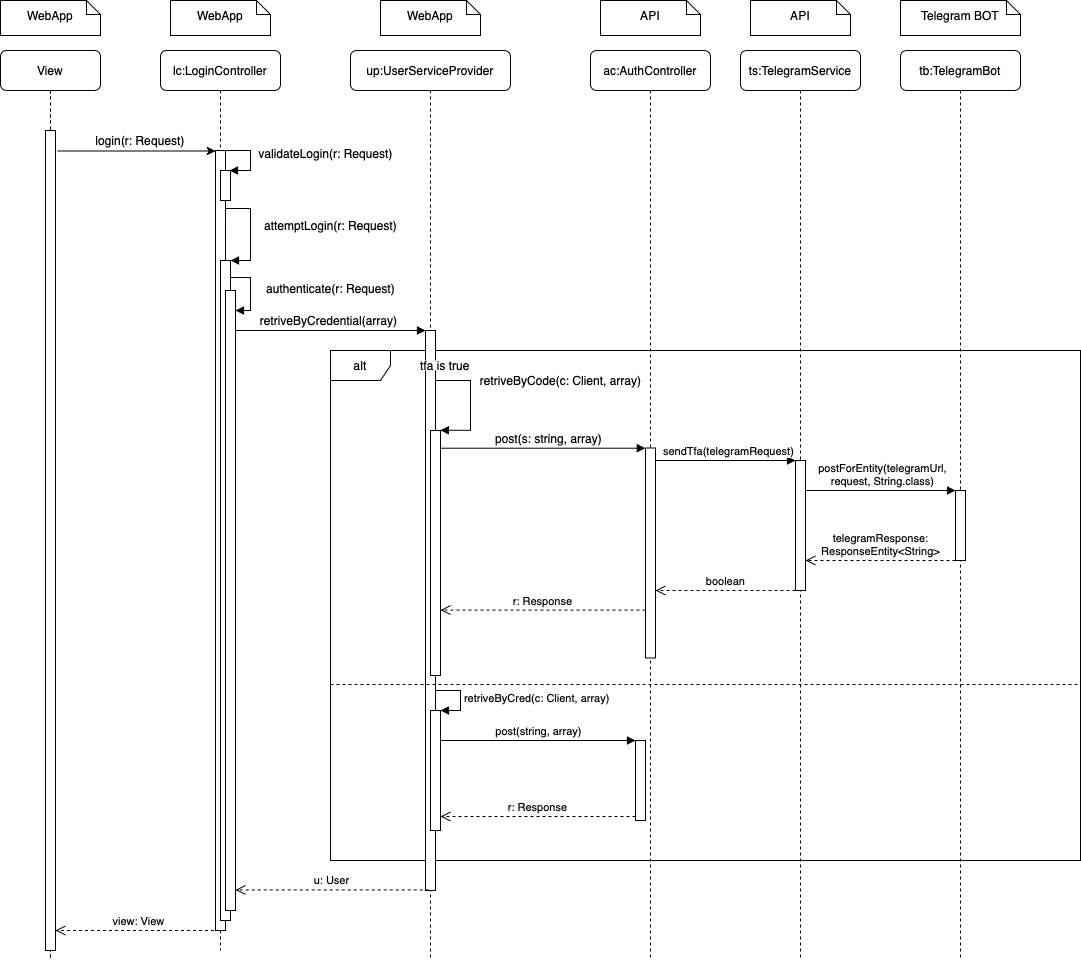
\includegraphics[scale=0.400]{res/images/WEBAPP/AutenticazioneTfa.png}
			\caption{Diagramma di sequenza che illustra l'autenticazione all'interno della componente web app}
			\label{Diagramma 23}
		\end{figure}
		Nel diagramma di sequenza che rappresenta l'autenticazione, alla richiesta della vista di effettuare l'autenticazione, il LoginController verifica che le credenziali siano corrette ed in seguito, se l'utente ha attivato l'autenticazione a due fattori, invia il codice tramite richiesta HTTP POST al bot di Telegram, il quale visualizza il codice nella chat dell'utente.
		\newline
		Mentre, se l'utente non l'ha attivata, invia semplicemente la risposta all'utente. In entrambi i casi viene mostrata la risposta affermativa o negativa all'utente e se positiva viene effettuata l'autenticazione.
		\begin{figure}[H]
			\centering
			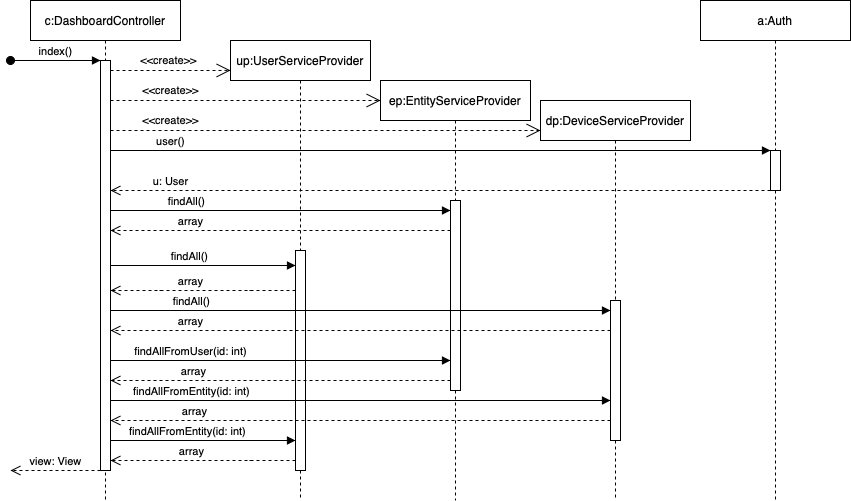
\includegraphics[scale=0.600]{res/images/WEBAPP/Dashboard.index.png}
			\caption{Diagramma di sequenza che illustra la visualizzazione della schermata dashboard all'interno della componente web app}
			\label{Diagramma 24}
		\end{figure}
		Come si evince dal diagramma, il DashboardController crea uno UserService, un EntityServiceProvider ed un DeviceServiceProvider, i quali effettuano le richieste \glock{API} per richiedere le informazioni da visualizzare nella dashboard, quali ad esempio il numero di utenti di un certo ente o le informazioni dell'account dell'utente che sta visualizzando la dashboard. Infine tutte le informazioni ricavate vengono restituite alla pagine view.
	\end{landscape}